\section{Evaluation}
\label{SEC:evaluation}


To evaluate \PPH, we evaluated the feasibility of its use 
in different scenarios.  This includes issues ranging from the efficiency
of the algorithm, to the expected security benefits from different 
configurations and deployment scenarios.  We frame our evaluation around
the following questions:

\begin{itemize}
    \item How long does \PPH take for different operations?
    \item What is the storage cost of \PPH?
    \item How much memory is needed for \PPH?
    \item What are the security properties of \PPH?
        \begin{itemize}
            \item What happens if users pick weak passwords?
            \item What \partialbytes settings should be used?
            \item How does the threshold affect the cracking time?
            \item What if a poor value is chosen for the threshold?
%            \item What is the feasibility of an attacker cracking a \PPH
%                protected store, with strong \thresholdaccount passwords
        \end{itemize}
\end{itemize}

%We will evaluate the time, memory and storage aspects of the algorithm and our
%python reference implementation. After this, we will analyze what are the
%optimal configuration values for \PPH by studying the behavior of the algorithm
%when we vary any of its parameters. Finally, we will summarize our findings and provide a
%case study to compare \PPH with regular salted hashes.

\subsection{What is the time cost of \PPH?}
\label{SUBSEC:time-costs}

To evaluate time costs, we examined how long it took PolyPasswordHasher to
process account verifications, new accounts, password changes, initializations
of a password store, and transitioning from bootstrapping to normal operation.
We measured the processing speed and performance of \PPH using an early-2011
MacBook Pro with 4GB of RAM and a 2.3 GHz Intel Core i5 processor.  All
operations reflect the mean verification time across 100 runs and were
performed with the password file already present in memory. For benchmarking
purposes, each action was performed sequentially despite being embarrassingly
parallelizable.

Figure~\ref{FIGURE:running-times} shows the time taken by different
operations (discussed below). Unless noted, the time cost of an operation did
not depend on other factors, such as the number of accounts in the password
database.

\paragraph{Time to verify an account} The mean time to verify a
\thresholdaccount was around 60$\mu$s independent of the threshold value.
For example, a threshold of eight allowed a server to verify more than 16K user
accounts per second.  Verifying a \thresholdlessaccount took approximately 29$\mu$s
and the server processed about 35K such actions per second. Bootstrap accounts,
which use salted hashing, took just over 3$\mu$s on the same platform.

The values presented do not include key stretching.  (Except for
the case of \partialverification, key stretching is unlikely to be used
for individual account verification with \PPH.)  
%At a minimum, we need to say we assume 1 billion hashes a second, if we
%assume that~\cite{ElcomSoftGPUCracking,zonenberg2009distributed}...


\begin{figure}
    \centering
    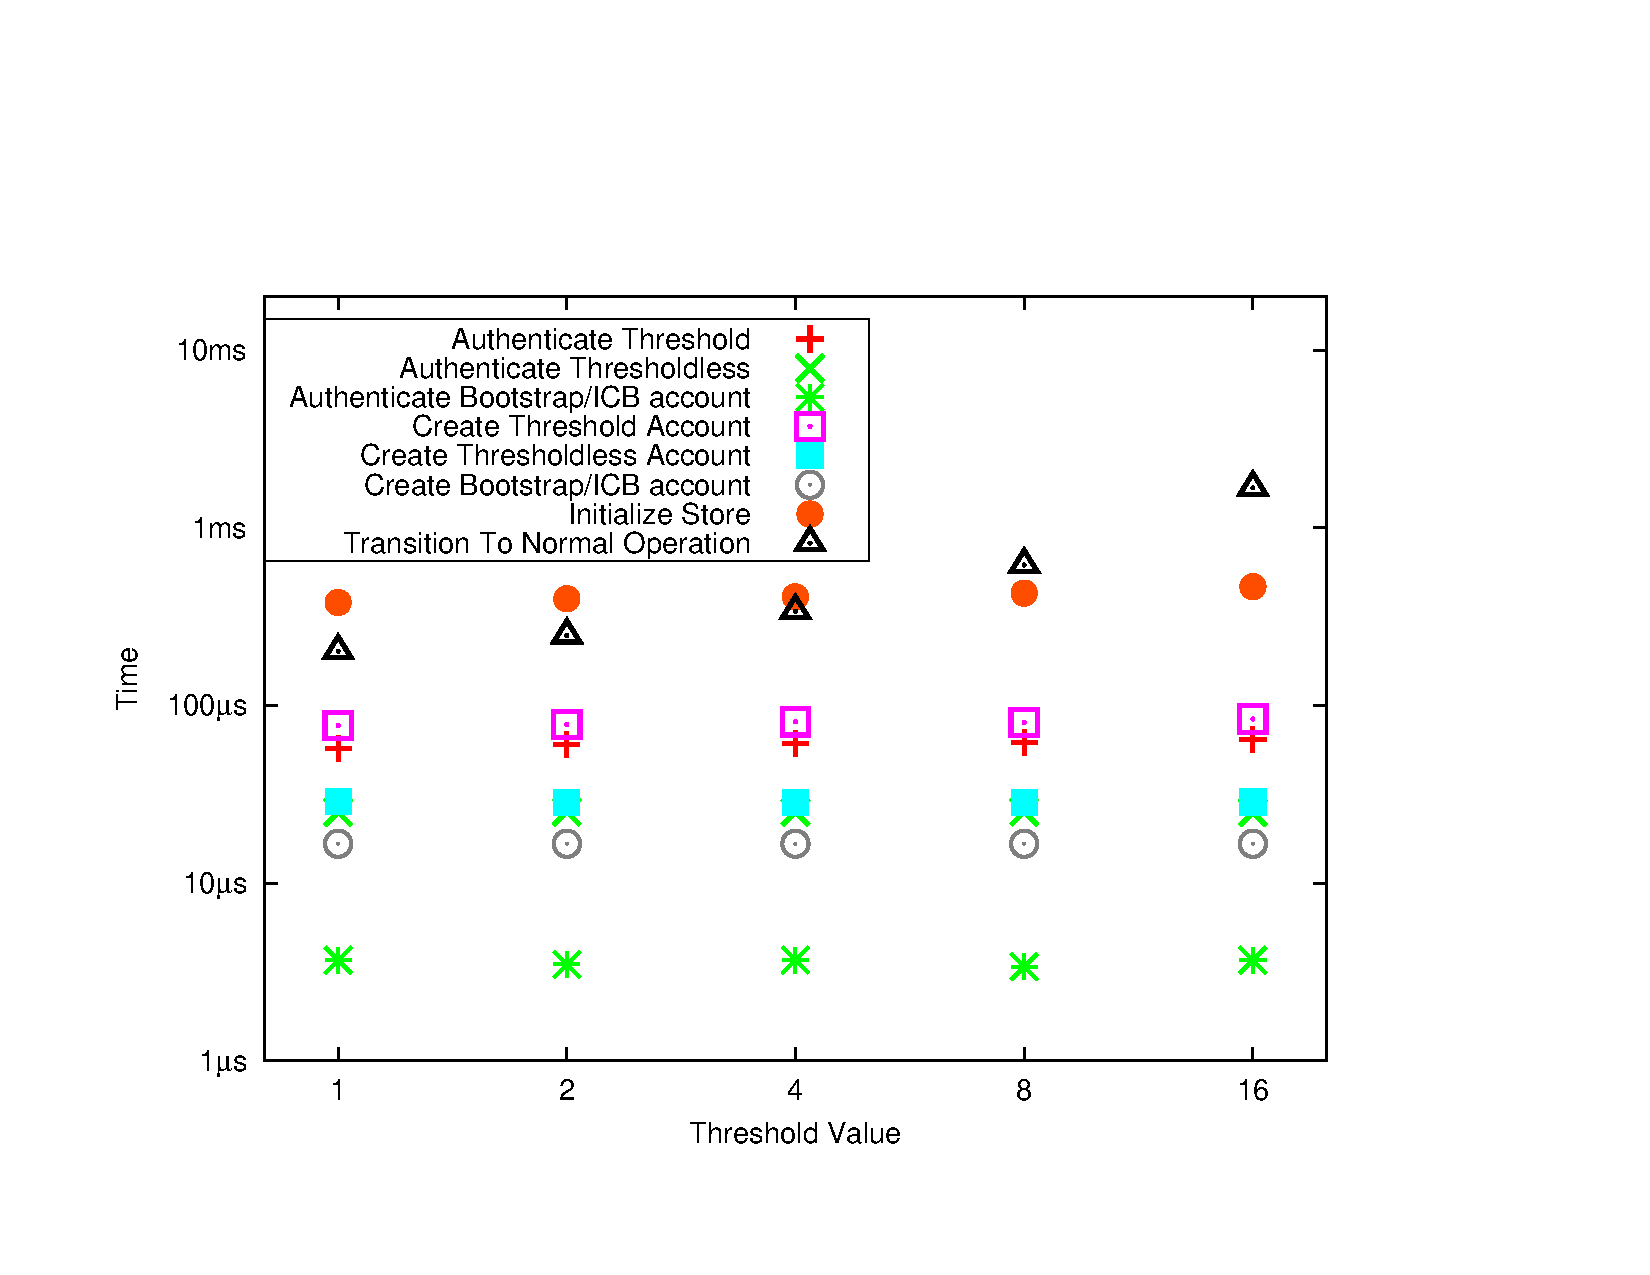
\includegraphics[width=.5\linewidth, trim=205 65 280 105]{./images/pph-running-times.pdf}
    \caption{Time needed per operations in \PPH. 
    \Partialbytes verification and transition to 
normal operation times are listed without key stretching.   }
    \label{FIGURE:running-times}
\end{figure}


\paragraph{Time to create accounts or process password changes}
Account creation time was similar to the time needed to verify accounts.
Depending on the threshold value, the average creation time varied from
77$\mu$s to 85$\mu$s. A \PPH store with a threshold value of eight created more
than 12K accounts per second. Given that there are a maximum of 255
\thresholdaccounts that can be created (at least with a \PPH implementation
that uses GF256), \thresholdaccount  creation time is not a performance
concern.  \Thresholdlessaccounts were created independent of the threshold, in
about 25$\mu$s. Based on this, we calculated that approximately 40K
thresholdless accounts can be created each second. This is similar to the time
it takes to generate a salted SHA256 hash for a password (16$\mu$s).  Changing
a password only requires \PPH to perform the same operation it uses to
create an account (and potentially also authenticate the old password).

\paragraph{Time needed to initialize a password database} The time to create a
database varied and was dependent on the threshold value used.  However,
varying the threshold from 2 to 16, varied the creation time from 380$\mu$s to
460$\mu$s. This time cost is largely due to the need to generate
cryptographically-suitable random numbers; but this operation is only
performed once, when a new password file is created.


\paragraph{Time needed to transition to normal operation} When the
server restarts, random coefficients are computed from the set of provided
shares, with full interpolation. The time needed to complete this operation
varied between 202$\mu$s and 1.6ms, because the threshold changes in relation to
changes in the number of polynomials, as the store size increases.  Note that
small thresholds were processed quickly --- a store with a threshold of 8 was
unlocked in 617$\mu$s.  There is also the time needed to do the integrity
check on the recovered secret.

Computing the random coefficients and computing the integrity
of the recovered secret (via a cryptographic hash) needs to be done once per 
restart for a normal server.  However, an attacker attempting to crack the
database will recompute the random coefficients and compute the hash once
per guess of \thresholdaccount values.  We therefore recommend that the 
integrity check use enough iterations of the hash function to increase the 
computational time needed to at least 100ms.   This slows the attacker
down per guess (a frequent operation), while only delaying the server slightly
one time per reboot.

{\bf Recommendation 1: The integrity check on the secret that is performed
when transitioning to normal operation should take at
least 100ms to complete.}

\subsection{What is the Storage Cost of \PPH?}

\begin{table}[t]
    \centering
    \renewcommand{\arraystretch}{1.3}

    \begin{tabular}{| c | c | c | c | c | c |}
    \hline
    {\bf Password } & {\bf Original} & {\bf Salted Hashes} & {\bf PPH }& {\bf PPH } & {\bf PPH }\\
    {\bf source} & {\bf space} & {\bf space} & {\bf No IV} & {\bf (16 ICB)} & {\bf (24 ICB)}\\
    \hline
    RockYou & 134MB & 260MB & 265MB & 275MB & 280MB\\
    \hline
    eHarmony* & 51.6MB & 100MB & 102MB & 106MB & 108MB\\
    \hline
    Formspring* & 27.3MB & 34.8MB & 35.2MB & 36.0 MB & 36.4MB\\
    \hline
    Gawker & 75.2MB & 119MB & 120MB & 122MB & 123MB \\
    \hline
    LinkedIn* & 252MB & 424MB & 430MB & 442MB & 448MB\\
    \hline
    Sony & 2.98MB & 4.95MB & 5.00MB & 5.10MB & 5.15MB\\
    \hline
    Yahoo & 17.8MB & 35.0MB & 35.4MB & 36.2MB & 36.6MB\\
    \hline
    \end{tabular}
    \caption{Disk space needed to store leaked password databases in
    different formats. * Denotes breaches in which only the salted hash portion
    of the database was released}
    \label{TABLE:disk-space}
\end{table}


%   ['eHarmony', 51.6, 100.0, 102.0, 104.0, 106.0, 110.0]
%   ['Formspring', 27.3, 34.8, 35.2, 35.60000000000001, 36.000000000000014, 36.80000000000002]
%   ['Gawker', 75.2, 119.0, 120.0, 121.0, 122.0, 124.0]
%   ['LinkedIn', 252.0, 424.0, 430.0, 436.0, 442.0, 454.0]
%   ['Sony', 2.98, 4.95, 5.0, 5.05, 5.1, 5.1899999999999995]
%   ['Yahoo', 17.8, 35.0, 35.4, 35.8, 36.199999999999996, 36.999999999999994]


Storing passwords with \PPH requires that additional information
-- a one byte share number -- be stored for each account.  This adds one byte
of storage space for each account, beyond the cost of current hash techniques.
The one byte has minimal impact on the disk space needed to store production
password databases (Table~\ref{TABLE:disk-space}).
% If \thresholdlessaccounts are stored in a
%separate file or are somehow distinguished stored independently, then only
%\thresholdaccounts require the extra byte of storage. This results in a cost
%for those accounts that is identical to the salted, hashed scheme. 

If the \partialbytes
field is used, the amount of information increases by the size of the field. 
For example, with a value of $24$ \partialbytes, the total cost increases by 
four bytes (one for the share number and three for the \partialbytes field). 

\subsection{How much memory is needed for \PPH?}

\PPH uses more memory than does a salted hash solution in normal operation.  
The server must store the polynomial coefficients for the 
Shamir Secret Share (which includes the secret).  However, the total size
of this data is relatively small --- the threshold value (2-5) multiplied by 
the length of the \sxh field (32 bytes).  As this value is likely to be
a few hundred bytes in practical deployments, (which is smaller than the \PPH 
code will be in memory), this should not pose a problem in practice.

During bootstrapping, additional memory is also used.  While shares are being
acquired, they are kept in memory.  This has a similar cost to storing
the polynomial coefficients for the Shamir Secret Share.
However, if \partialverification is used, the more
substantial cost is storing authentication information so that it can be
verified against the complete entry to ensure that the previous login was
correct. The memory cost of caching this information will correspond to the
number of logins before bootstrapping is finished (i.e., \sxh * Log-ins).
The total memory cost is still rather small, even for a server that processes
many authentications.  For example, a server that processes ten thousand logins
while bootstrapping needs only 320KB of memory to store that information.  Thus
the memory costs remain small, even for heavily used systems.
 


\subsection{What happens if users choose extremely weak passwords?}
\label{SUBSEC:bad-passwords}

If extremely weak passwords are
used for a threshold of \thresholdaccounts (like administrators), \PPH will not
provide strong protection.   If there are only a few bits of entropy in the
password, the search space will still be small, but exponentially larger.   
For example, if the attacker knows that three \thresholdaccounts each chose one
of 10 weak passwords, the attacker could sweep the search space in 1000
guesses (100 seconds, given a 100ms time to verify the secret).  While this
is much better than the 30 guesses an attacker would need with salted hashing,
this protection is obviously still very weak.  It
is thus critical that \thresholdaccounts are secured with strong passwords.  
\PPH performs very poorly when weak passwords are used for \thresholdaccounts.  Even 
with extremely weak passwords, \thresholdlessaccounts will have some 
protection, so long as the \thresholdaccounts use strong passwords.  

However, independent of any storage technology, extremely weak passwords 
are susceptible to guessing by an external party without having to steal
the password database.  Therefore, this is not an area that password database
storage technologies can address.

Fortunately, research has shown that users can be helped to choose passwords
that have a significant degree of randomness.  This can be done by requiring a combination of
passwords that are a certain length (8 characters), combinations
of character types (letters, numbers, symbols), and by blacklisting common
passwords~\cite{weir2010passwordpolicies}.  Extremely weak passwords are
susceptible to guessing by an external party (without database access); as
best practice, sites should block them from use~\cite{bancommonpasswords,
weir2010passwordpolicies, cormac2014telepathwords,
kelley2012guessingpasswords}.  The combination of length, diverse character
types, and blacklisting common passwords has been shown to substantially
increase the time needed to crack passwords.

%We applied these techniques to passwords from the RockYou password dump
%and then evaluated the entropy of the resulting password entries.  We 
%found ...\cappos{Continue in this vein with results...}
%Thus we expect the \thresholdaccounts can
%pick passwords with ?? bits of entropy; equivalent entropy to
%a ????-character-long, random password.


{\bf Recommendation 2: \Thresholdaccounts should have
as much entropy as a 6-character-long random password.}


%However, \PPH provides the ability to protect \thresholdlessaccounts even if they do not
%pick good passwords, for they are protected by the \thresholdaccounts. When an
%attacker attempts offline cracking on a \PPH-enabled database, his only
%alternative is to crack different \thresholdaccounts simultaneously first, and then
%crack the whole database as he would do against regular salted hashing. 


\subsection{{\bf What \partialbytes setting should be used?}}
\label{SUBSEC:security-properties}

%\cappos{Throughout the paper, we need to be sure we don't say 
%\partialbytes = 0, when we mean disabling \partialverification.  
%We never mean \partialbytes = 0.  We should always say disabling instead.}

\Partialverification changes the properties of \PPH, depending on the
size of the \partialbytes field.  
\begin{itemize}

\item When \partialverification is disabled, a user may not log in until a
threshold of \thresholdaccount passwords have been provided.  This makes \PPH
unavailable during the bootstrap phase.  

\item When the size of the \partialbytes field is very small, 
it is possible that authentication errors will be made during bootstrapping.
For example, if the size of the \partialbytes field is set to 1 bit (an
implausible and extreme example), then an attacker typing a random password 
has a 50\% chance of the \partialbytes matching and being allowed in.

\item  As the size of the \partialbytes field grows, the probability that an
attacker will succeed with online cracking decreases. However, when the size of the
\partialbytes field is very large, if an attacker steals the database, the
confidentiality benefits of \PPH are weakened.  For example, in the extreme
case that the \partialbytes field is the size of the entire salted password
hash (an implausible example), then an attacker can use the slow,
\partialverification hash to individually crack passwords.  In this case, from
a security standpoint, \PPH is effectively equivalent to key stretching.  The
primary benefit of \PPH in this case is that it does authenticate accounts much
more quickly in normal operation than does key stretching.

\end{itemize}

Given that the size of the \partialbytes field and the threshold is
configurable, the security properties of \PPH vary. When integrating \PPH into
a system, an administrator can leverage this adaptability to better meet his
expectations.  In the next subsection we explain how different configurations 
of \PPH apply to different use cases.


\begin{figure}
    \centering
    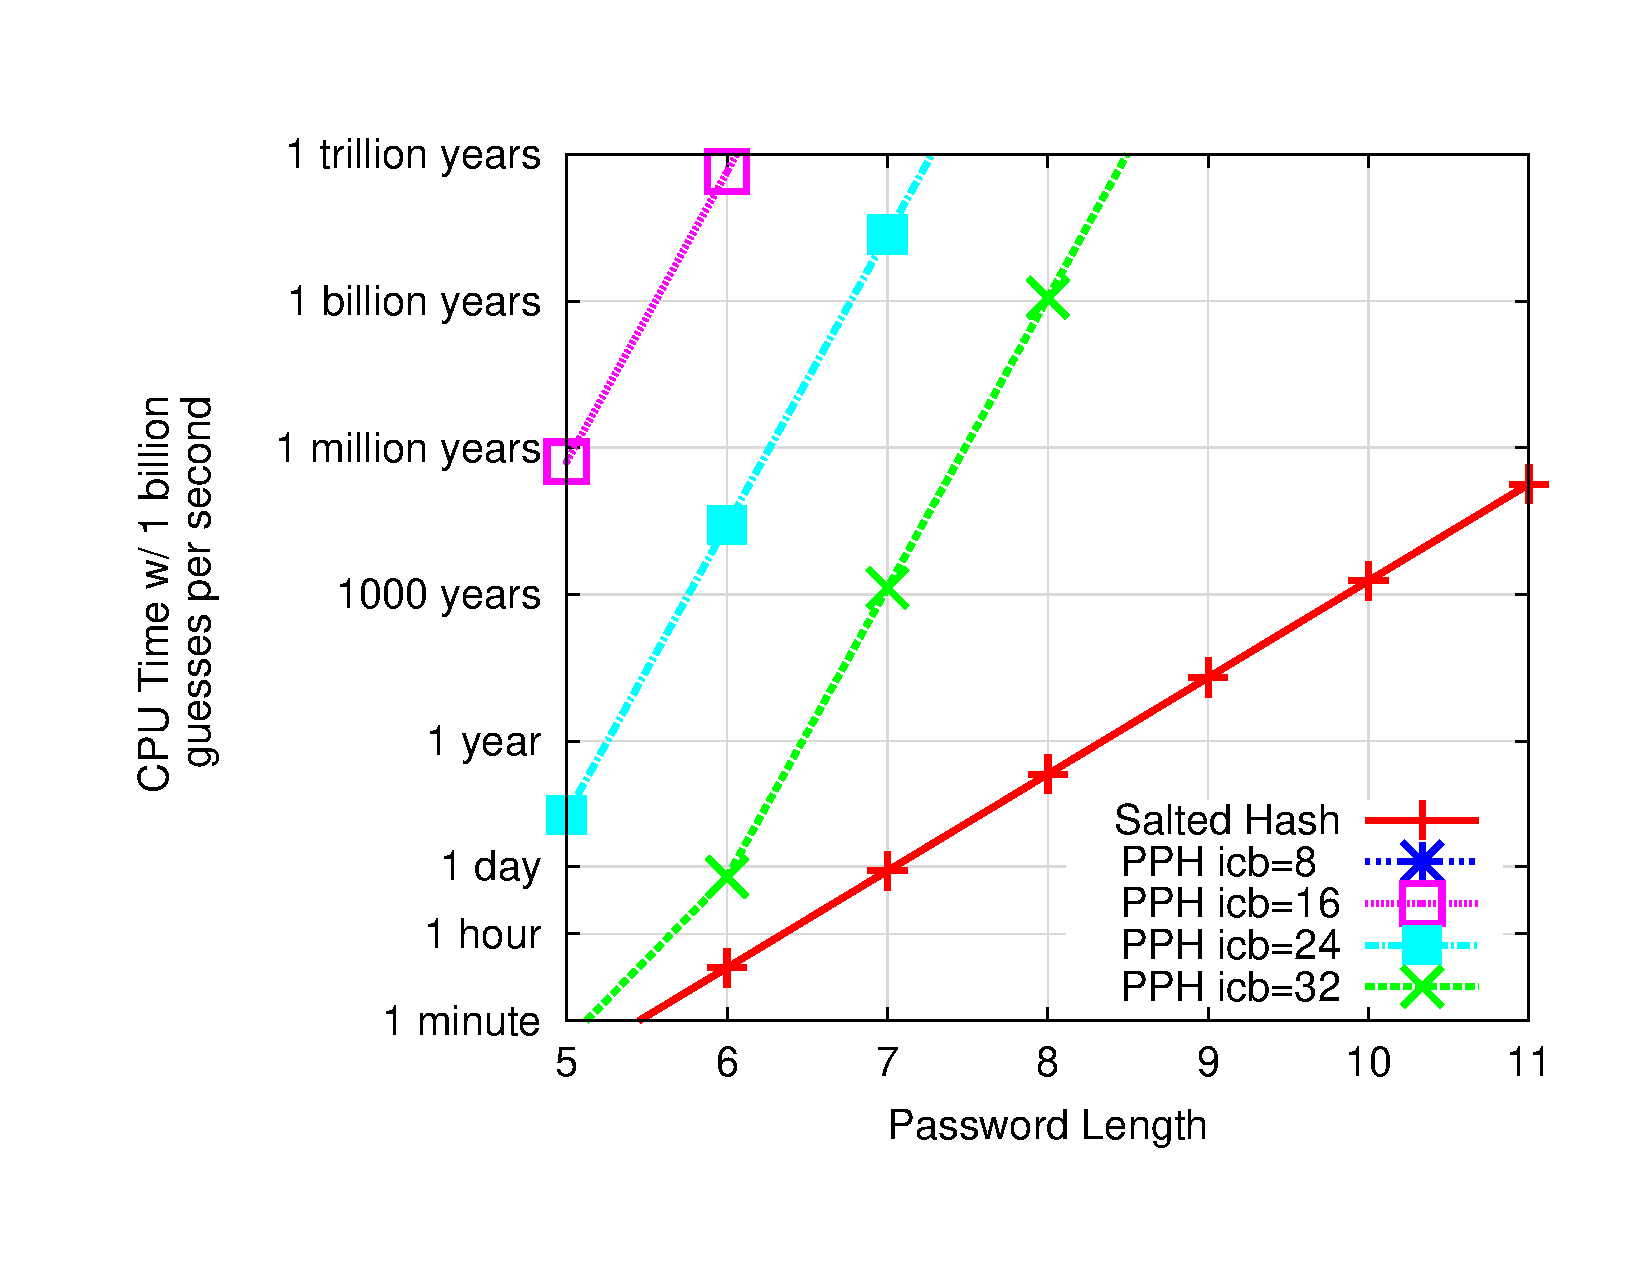
\includegraphics[width=.5\linewidth, trim=195 55 165 55]{./images/plotcrack_icb}
    \caption{{\small Time it takes to crack a \PPH store with different values
    for \partialbytes and a threshold of 3.  The line for \partialbytes=8
does not fit within the axes of the graph. }}
    \label{FIGURE:cracking-icb}
\end{figure}



\subsubsection{Immediate Availability For Many Unknown Clients}
In some situations, after
reboot a server needs to be immediately available to a potentially huge 
number of untrusted clients.  For example, a 
web forum or a social media site is likely to have this property.
Availability is paramount, for a large, diverse, and constantly changing
user base.

If an attacker has his attack detected and his IP address blocked, this 
may not be a major concern or deterrent. Therefore, attackers may try to do things such as
brute force passwords, even if this is likely to lead to detection.

There is also a risk of users trying incorrect passwords during the bootstrap
phase to try to break into an account.  Most existing web frameworks deal with
this by restricting the number of password attempts from an IP address over a
period of time (10 authentications per second is common).  However, a motivated
attacker with the ability to connect from many IP addresses (e.g., a botnet
operator), could still be able try a substantial number of passwords.
However, using a \partialbytes value of 24 bits will cause the attacker's
password search space to be as large as the usual number of attempts for
successful online cracking scenarios.

% \cappos{probably discuss somewhere here how bootstrapping is only used
% for a short time..}



The downside is that a large \partialbytes field will make it easier for an
attacker to crack the \thresholdaccounts.  As shown in
Figure~\ref{FIGURE:cracking-threshold}, as the size of the \partialbytes field
grows, the cracking time for a threshold of three starts to resemble the time
for salted hashes. For 24 \partialbytes, the time to crack a six-character
equivalent random password is around $270420$ years. In summary, the
\partialbytes setting reduces the password entropy.  To provide adequate
protection, either passwords with the entropy of 8 character random passwords
should be used, or, as will be discussed later, the threshold should be
increased.


{\bf Recommendation 3: In situations where a large number of unknown clients
will authenticate, use a setting of 24 \partialbytes.}


\subsubsection{Immediate Availability For Known Clients}
In many cases, the set of expected clients is limited and known.
This includes situations like a institutional file server or mail server.
In this case, the total set of possible clients is limited and it is
assumed that an attacker cannot control a large number of IP addresses / 
clients.

\begin{table}[t]
    \centering
    \renewcommand{\arraystretch}{1.3}

    \begin{tabular}{| c | c | c | c |}
    \hline
    {\bf guessing} & \multicolumn{3}{ c|}{{\bf Attempts}} \\  
    {\bf probability} & {\bf ICB=8} & {\bf ICB=16} & {\bf ICB=24} \\ 
    \hline
    25\% & 76 (25.4\%) & 18,767 (24.9\%) & 4,804,150 (24.9\%) \\
    \hline
    50\% & 177 (49.9\%) & 45,295 (49.9\%) & 11,595,559 (49.9\%) \\
    \hline
    75\% & 354 (74.9\%) & 90,590 (74.9\%) & 23,191,185 (74.9\%) \\
    \hline
    \end{tabular}
    \caption{Number of attempts required to find a \partialbytes collision}
    \label{TABLE:collisions}
\end{table}



%   []    [8.0, 16.0, 24.0, 32.0]
%   ['25.0%', '100(0.32388353489%)', '18767(0.249010703106%)', '4804150(0.249000026671%)', '99999999(0.0230141050386%)']
%   ['50.0%', '177(0.499806462193%)', '45295(0.499001475831%)', '11595559(0.499000008952%)', '99999999(0.0230141050386%)']
%   ['75.0%', '354(0.749806424736%)', '90590(0.74900047878%)', '23191185(0.749000011343%)', '99999999(0.0230141050386%)']

In this case, an attacker who brute forces accounts is much less of a concern
because he cannot obtain the IP addresses needed and failed attempts should
be flagged and investigated by the security team regardless.  Thus, setting
\partialbytes to be 16 requires that an attacker attempt to crack $45295$ passwords to
have a probability of finding a collision of about 50\%, as shown in
Table~\ref{TABLE:collisions}. This configuration is ideal for cases in which a
lock-out policy can be enforced. However, even if an attacker was able to find
a collision during bootstrapping, \PPH would be able to detect it upon
recombination. If an attacker were to find a collision when \PPH is performing
on normal operation, then the break-in attempt would also notify the
administrators.


The bigger concern is an attacker (possibly an insider) stealing the database 
and brute forcing account passwords.   By using a small number of 
\partialbytes, such as 16, the resilience to cracking is very high.  Even 
if there are three \thresholdaccounts with the entropy of a 6 character
password, it would require $447.8 * 10 ^ 6$ thousand years of CPU effort to crack these
accounts.


{\bf Recommendation 4: In situations where a restricted set of clients will
try to authenticate, use a setting of 16 \partialbytes.}


\subsubsection{When Short Periods of Unavailability are Acceptable}

In some situations, temporary unavailability of a server (while bootstrapping)
is not a major concern.  For example, many services load balance 
requests across multiple systems for redundancy and performance.  
Administrators will stop and start instances as needed.  When starting
an instance, the first thing the administrators will typically do is log into
the system to validate that it is working, before moving it into production.
For such a system, the time spent in the bootstrapping phase is small
and there is no user-perceived unavailability while the system is 
bootstrapping.

In this case, \partialverification can be completely disabled, maximizing
the security benefit of \PPH.  The CPU time it would take an attacker to crack 
the database is infeasibly high for practical situations.  
Even with a threshold of 3 and 5 character random accounts, the cracking time 
when \partialverification is disabled ($1.46*10^{21}$ CPU years) extends past the 
top of the y-axis 
in Figure~\ref{FIGURE:cracking-icb}.  (This is more CPU time than would be 
provided by every computer working nonstop for the estimated 
age of the universe.)   Thus, given our understanding of the security of
SHA256 and AES, it is infeasible for any adversary to use the password
database to crack passwords with the entropy of 5 character random
passwords that are stored in this manner.

%\cappos{Low priority: Add a table or similar...}
\begin{table}[t]
    \centering
    \begin{tabular}{ | c | c | c | c | c |}
        \hline
        {\bf Equivalent} & \multirow{2}{*}{{\bf ICB}} & \multirow{2}{*}{{\bf Threshold}} &
        \multirow{2}{*}{{\bf Keyspace}} & \multirow{2}{*}{{\bf Recombinations}} \\
        {\bf Entropy} & & & & \\
        \hline
        \multirow{6}{*}{\parbox[h]{1.8cm}{\centering 32.45 \\(5 character-long,\\ random password)}}
        & \multirow{2}{*}{Disabled} & 3 & $4.632*10^{29}$ & $5.559*10^{31}$ \\ 
                                \cline{3-5}
                                &    & 4 & $3.584*10^{39}$ & $7.528*10^{41}$ \\
                                \cline{2-5}
                               & \multirow{2}{*}{16} & 3 & $1.645*10^{13}$ & $1.975*10^{17}$ \\
                                \cline{3-5}
                               &    & 4 & $1.943*10^{18}$ & $4.080*10^{22}$\\
                                \cline{2-5}
                               & \multirow{2}{*}{24} & 3 & $2.331*10^{10}$ & $1.175*10^{10}$\\ 
                                \cline{3-5}
                               &    & 4 & $7.619*10^{10}$ & $9.484*10^{12}$\\ 
        \hline
        \multirow{6}{*}{\parbox[h]{1.8cm}{\centering 38.85\\(6 charater-long,\\ random password)}} 
        & \multirow{2}{*}{Disabled} & 3 & $4.972*10^{35}$& $6.554*10^{37}$ \\ 
                                \cline{3-5}
                                &    & 4 & $2.919*10^{47}$ & $9.635*10^{49}$ \\
                                \cline{2-5}
                                & \multirow{2}{*}{16} & 3 & $1.411*10^{21}$ & $1.693*10^{23}$ \\ 
                                \cline{3-5}
                                &    & 4 & $1.582*10^{28}$ & $3.24*10^{30}$ \\ 
                                \cline{2-5}
                                & \multirow{2}{*}{24} & 3 & $8.631*10^{13}$ & $1.009*10^{16}$ \\ 
                                \cline{3-5}
                                &    & 4 & $3.684*10^{18}$ & $7.738*10^{20}$ \\ 
                                \cline{2-5}

        \hline
        \multirow{6}{*}{\parbox[h]{1.8cm}{\centering 45.21\\(7 character-long,\\ random password)}} 
        & \multirow{2}{*}{Disabled} & 3 & $3.405*10^{41}$ & $5.619*10^{43}$ \\ 
                                \cline{3-5}
                                &    & 4 & $2.378*10^{55}$ & $7.848*10^{57}$ \\
                                \cline{2-5}
                                & \multirow{2}{*}{16} & 3 & $1.209*10^{27}$ & $1.558*10^{28}$ \\ 
                                \cline{3-5}
                                &    & 4 & $1.289*10^{36}$ & $2.976*10^{50}$ \\ 
                                \cline{2-5}
                                & \multirow{2}{*}{24} & 3 & $7.211*10^{19}$ & $8.654*10^{21}$\\ 
                                \cline{3-5}
                               &    & 4 & $3.685*10^{26}$ & $6.303*10^{28}$ \\ 
                                \cline{2-5}

        \hline

    \end{tabular}
    \caption{{\small Equivalent keyspaces and number of recombinations for
    different \PPH configurations. Assuming 10 \thresholdaccounts}}
    \label{TABLE:pph-configurations}
\end{table}


%It is important to consider that disabling \partialverification affects the
%availability of the system, since it cannot provide account verification
%until the server has finished bootstrapping.

{\bf Recommendation 5: In situations where availability immediately
after a reboot is not essential, \partialverification should be disabled.}

\subsection{How does the threshold affect the cracking time?}
\label{SUBSEC:threshold-value}


The threshold value is directly related to the cracking time by
increasing the number of secret recombinations that an attacker needs
to attempt before he can recover the secret. Also, on the usability side,
it is also related to the time it takes for a system to transition
from the bootstrap phase to normal operation.  

We can see in Figure~\ref{FIGURE:cracking-threshold} that, when we fix the
\partialbytes number to 24, the threshold value exponentially increases the cracking time. 
(We choose a high number of \partialbytes because the
security is lower and thus, differences are easier to see on the graph.)
If the \thresholdaccounts pick strong enough passwords, and the 
threshold is three, the cracking time increases by many orders of magnitude.
The regular salted hashes are expected to be cracked in about 40 minutes,
whereas, if using \PPH, these hashes would be cracked in $27,042$ years.

The reason why \PPH provides strong protection is that
even when an attacker has to guess only a few passwords, in most cases \PPH's
exponential increase in guessing time ($O(Vp)$ instead of $O(pV)$, will make
guessing a password computationally infeasible
(Figure~\ref{FIGURE:cracking-threshold}). 
Furthermore, it is possible to much more aggressively apply a technique like 
key stretching for the integrity check of the reconstructed secret.  This is
because this operation is only done once (by the server), but is done for
each guessed combination of passwords (by the attacker).  This increases
the attacker's time cost while extending the time the server spends, by a second or less, in 
bootstrapping .

%For example, suppose an attacker wants to
%guess three passwords that he knows are each comprised of six randomly chosen
%characters. Recent studies have shown that a GPU can compute on the order of a
%billion password hashes per second
%~\cite{ElcomSoftGPUCracking,zonenberg2009distributed}, thus allowing an
%attacker to search the key space for all three passwords in under an hour,
%which indicates that the current state of the art provides little protection
%against password guessing.
%
%Even a threshold of two provides substantially stronger protection than do
%existing best practices. Searching the key space would require over 17 million
%CPU years of effort.

{\bf Recommendation 6: Choose a threshold of 3 plus the number of 
\thresholdaccount passwords an attacker could reasonably know, for strong 
protection.}



\begin{figure}
    \centering
    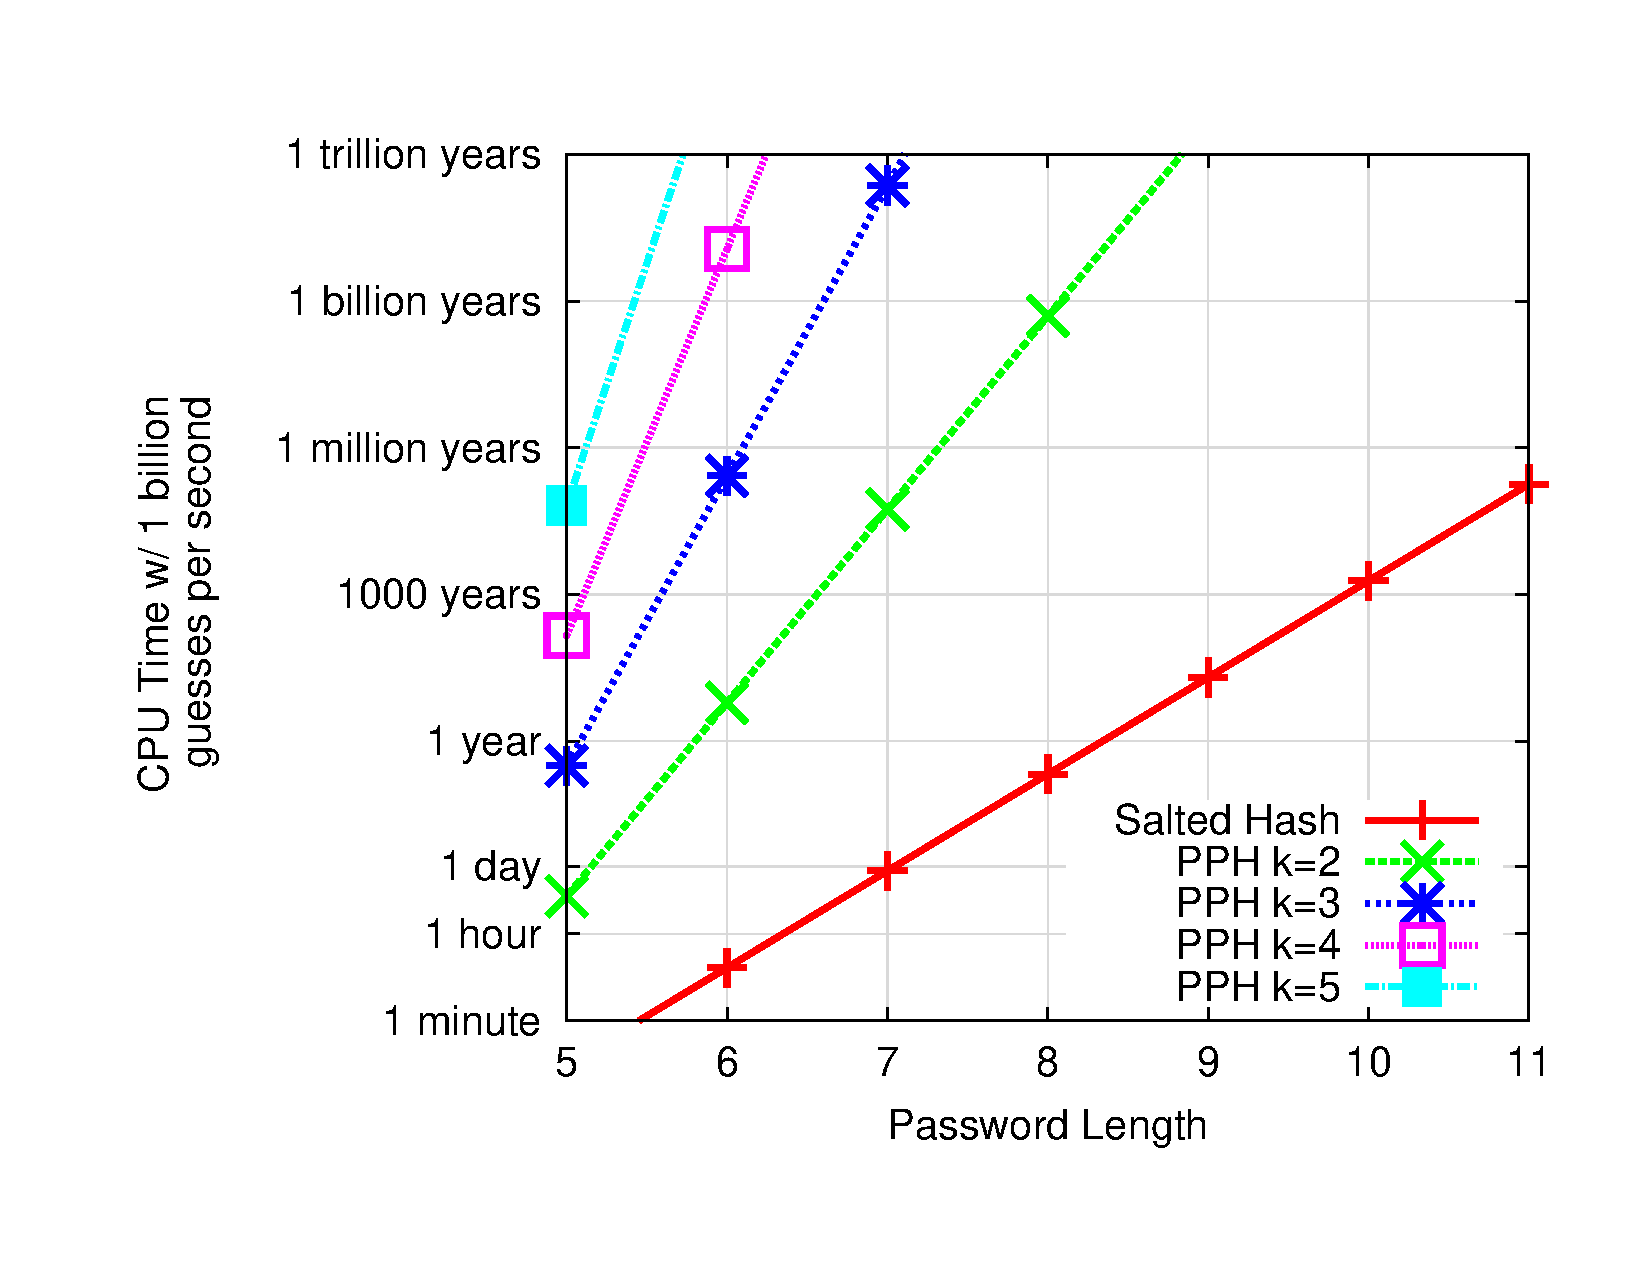
\includegraphics[width=.5\linewidth, trim=195 55 165 55]{./images/plotcrack_threshold}
    \caption{{\small Time it takes to crack a \PPH store with different values of 
    threshold and 24 \partialbytes}}
    \label{FIGURE:cracking-threshold}
\end{figure}

\subsection{What if a poor value is chosen for the threshold?}

Choosing a poor threshold setting can minimize the protections of \PPH.
If the threshold is too high, the system will primarily be in the 
bootstrapping phase while waiting for \thresholdaccounts to log in.  
Thus most of the accounts will be bootstrap accounts and only be protected 
by salted hashes.  If an attacker steals this database, they can individually 
crack these passwords.

An organization might find that there are not enough \thresholdaccount logins to get
the system into normal operation.   One way to mitigate this is to promote 
some \thresholdlessaccounts that log in frequently to be \thresholdaccounts.  
This would allow an attacker who controls one or more of those accounts to
have an easier time cracking the \thresholdaccounts, but causes bootstrapping
accounts to be protected.

{\bf Recommendation 7: It is often better to have \thresholdaccounts that 
frequently log in (but who are untrusted), than those of trusted users
who rarely log in.} 

If the threshold setting is too low, then an attacker can feasibly crack
the \thresholdaccounts and gain the ability to individually crack accounts.
This is particularly problematic when combined with a large \partialbytes
settion.  The minimum threshold setting described in the previous
settings should be used wherever possible. This relationship can be verified 
by consulting Table~\ref{TABLE:pph-configurations}



%\cappos{I'm of the opinion we should cut the Sony Breach.  Given time, we 
%could do an analysis of the RockYou database with the passwords that pass our
%filters.   (Entropy eval then look at this.)
%
%I don't think this helps our case and the argument about why we don't toss
%things is muddied by our other arguments...
%}

\eat{
\subsection{Case study: the Sony Breach}
\label{SUBSEC:sony-database}

To explore how these results carry over to real passwords, we performed an
experiment using the password data dumped from the Sony account
breaches~\cite{sonyhack}.  Of the leaked password databases known to the 
authors (Table~\ref{TABLE:disk-space}), this is the only data set which 
explicitly lists which accounts are administrator accounts versus normal users.

\santiago{this should be revised, what if we throw away the weak passwords}
In the database dump, there is password data for both outside user accounts as
well as accounts have administrator access. The four administrator accounts
have passwords with the estimated entropy in bits~\cite{passwordstrength}:
password@1 (5.322 bits), welkom@1 (26.553 bits), waderobsen (30.618 bits), and
itsafullcyrcle (44.011 bits). Given a rate of a billion password hashes checked
per second, the first three passwords can all be cracked in two seconds. The
remaining password (and thus every administrator password) could be cracked in
under 5 hours.

If \PPH were protecting these passwords, the ability to crack the
passwords would depend on the threshold. The effective password strength is
that of the weakest passwords combined, times the probability of selecting
those accounts in that order. A threshold of 3 will have an effective entropy
of 67.078 bits, which will take nearly 5000 years to crack, based on 1 billion
guesses per second.

With a threshold of 2, the effective entropy is 35.459 bits, which can be
cracked in under a minute. However, if all administrators chose a password as
strong as the password waderobsen (which is considered a weak password by
current standards~\cite{passwordstrength}), then the password would have had an
effective entropy of 64.820 bits, and take more than a thousand CPU years to
crack at 1 billion guesses per second. This underscores the fact that
administrators still should not choose immensely poor passwords (e.g.,
‘password@1’).  Independent of password storage concerns, avoiding trivially
guessable passwords is essential in preventing remote brute-force password
cracking.

\Thresholdlessaccount passwords (many of which tend to be extremely weak) cannot
be cracked until a threshold of administrator passwords are compromised. This
means that even it is only administrators who can be convinced to use strong
passwords, \PPH still provides substantial security benefits.


\eat{
\santiago{This is part of the old eval, we can take information from here}
\Partialverification allows an attacker to first reduce the search space for a
specific account by eliminating accounts that do not match the leaked bits. If
the attacker knows the password pattern, he can first precompute all passwords
that match that pattern and hash. This requires the same amount of effort
(k*2n) as for cracking passwords that are stored using traditional best
practices. If the attacker has sufficient space to store these passwords, he or
she may then use combinations of these precomputed passwords to try to unlock
the database. The attacker will be able to search the space for the Shamir
Secret Store in 2k*n-l guesses.  Each byte used for \partialverification
effectively reduces the strength of a random password by approximately 1.22
characters. However, the time needed to unlock the Shamir Secret Share still
represents an exponential increase and dominates the overall cost.

With one billion operations per second, sweeping the search space would still
require 45 thousand CPU years (8 orders of magnitude more time than salting and
hashing).  For example, if 2 bytes are leaked for 6 random character passwords
(Figure~\ref{FIGURE:cracking-times}), the attacker will need to do 735 trillion
operations for each of the three passwords and then 1.41×1021 operations to
crack the password database. 
}
\subsection{Summary}
\label{SUBSEC:summary}
}
